\chapter{LCA*}
\label{chap:lca*}

In dit hoofdstuk leggen we eerst het algemene concept van de lowest common
ancestor (LCA) uit. We bekijken de verschillende toepassingen van dit concept in
de biologie en lichten toe hoe dit LCA algoritme wordt gebruikt in
Unipept. Na deze inleiding stellen we een variant van dat algoritme voor,
LCA*, en leggen we uit waarom LCA* in sommige gevallen een specifieker
resultaat oplevert dan algemene LCA. Hierna diepen we een zeer snelle
implementatie van het originele LCA algoritme uit, tonen we aan hoe we dit
algoritme kunnen uitbreiden tot een algoritme voor LCA* en lossen we enkele 
problemen op die die uitbreiding met zich meebrengt. We sluiten af met een
voorbeeld van hoe LCA* zou kunnen worden ingebouwd in de Unipept webservices.

\section{Inleiding}
Het lowest common ancestor (LCA) probleem is een klassiek probleem in de
grafentheorie. De LCA in een boomstructuur wordt gedefinieerd als de
gemeenschappelijke ouder van twee (of meer) nodes die zich het verst van de
wortel bevindt. Toegepast op het voorbeeld in \Vref{tikz:lcavoorbeeld}, kunnen
we bijvoorbeeld de LCA berekenen van node E en J. Nodes waarvan we de LCA
berekenen, zullen we in het vervolg ``querynodes'' noemen. Volgens de definitie
hierboven is de LCA van E en J gelijk aan C. De notatie die we hier in het
vervolg voor zullen gebruiken is: LCA(E, J) = C. Wanneer we de LCA berekenen van
twee nodes op hetzelfde pad, resulteert dit in de node dichtst bij de wortel,
zoals te zien is op \Vref{tikz:lcadg}.

\begin{figure}
    \centering
    
    \begin{subfigure}{0.45\linewidth}
        \centering
        \begin{tikzpicture}[node distance=3cm, level distance=1.5cm,
            every node/.style={draw, thick, circle,inner sep=5pt},
            every path/.style={->, draw, thick, -latex'}]
        \Tree [. A 
                 [. B ]
                 [. \node[draw, fill=red]{C};
                    [.\node[draw, fill=yellow]{E};
                       [. H ]
                       [. I ]
                    ]
                    [. F
                       [. \node[draw, fill=yellow]{J}; ]
                    ] 
                 ]
                 [. D
                    [ . G ]
                 ] 
              ]
        \end{tikzpicture}
        \caption{}
        \label{tikz:lcaej}
    \end{subfigure}
    \begin{subfigure}{0.45\linewidth}
        \centering
        \begin{tikzpicture}[node distance=3cm, level distance=1.5cm,
            every node/.style={draw, thick, circle,inner sep=5pt},
            every path/.style={->, draw, thick, -latex'}]
        \Tree [. A 
                 [. B ]
                 [. C
                    [. E
                       [. H ]
                       [. I ]
                    ]
                    [. F
                       [. J ]
                    ] 
                 ]
                 [. \node[draw, fill=red]{D};
                    [ . \node[draw, fill=yellow]{G}; ]
                 ] 
              ]
        \end{tikzpicture}
        \caption{}
        \label{tikz:lcadg}
    \end{subfigure}
                
    \caption{Bovenstaande figuren worden twee voorbeelden getoond van het
    algemene LCA concept. Links nemen we de LCA van node E en J, met C als
    resultaat. Rechts berekenen we de LCA van twee nodes op hetzelfde pad, D en
    G. Dit geeft de node dichtst bij de wortel als resultaat, namelijk D. Nodes
    in het geel zijn de nodes waarvan de LCA wordt berekend, de rode nodes zijn
    het resultaat van de LCA bewerking.} 
    \label{tikz:lcavoorbeeld}
\end{figure}

Binnen de (meta)proteomics wordt de berekening van de LCA ook vaak gebruikt. Dit
wordt geïllustreerd in \Vref{fig:workflow} waar in de laatste stap de LCA
genomen wordt van alle gevonden taxa in de Unipept taxonomy.

\begin{figure}
	\centering
    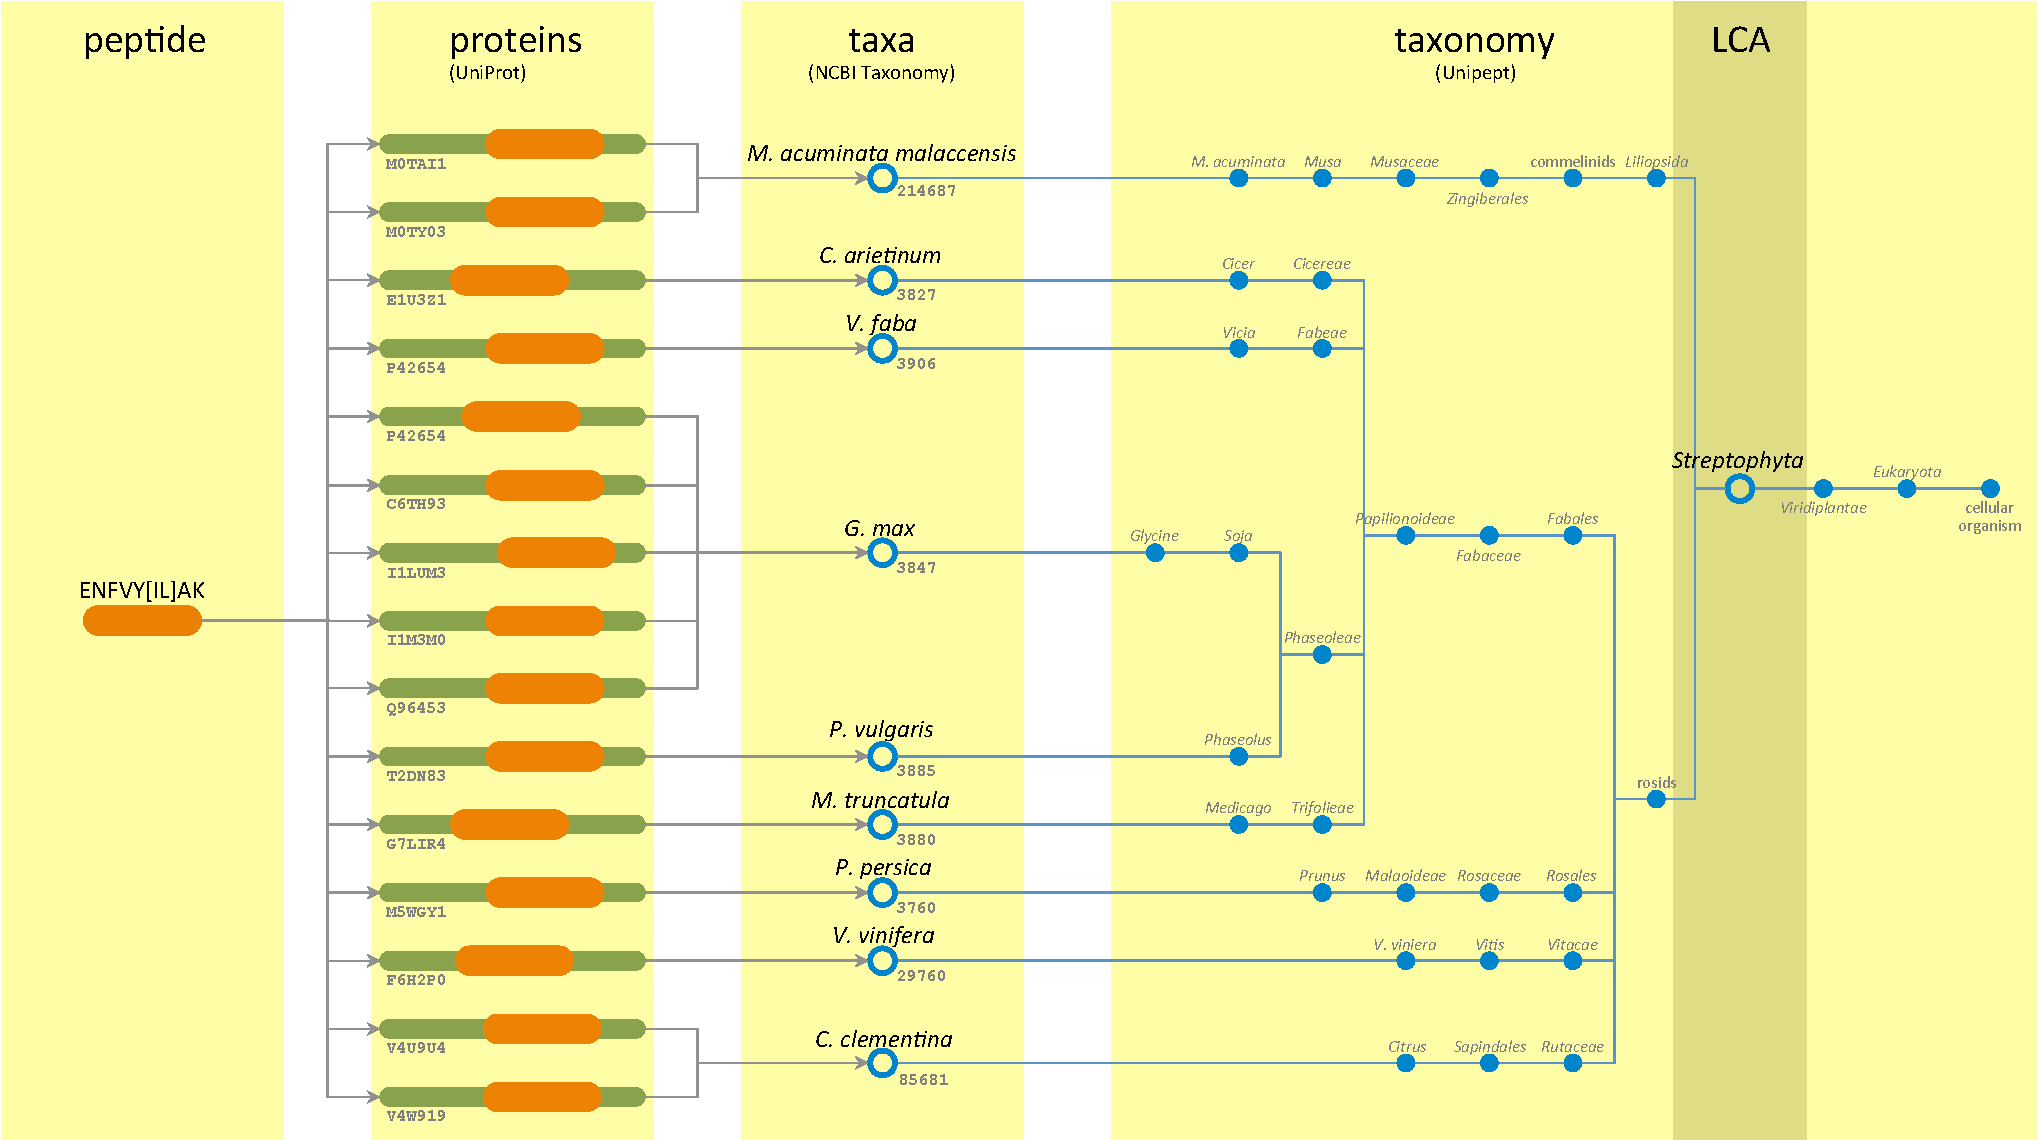
\includegraphics[width=0.8\textwidth]{includes/workflow}
    \caption{Illustratie van het gebruik van lowest common ancestor binnen de 
    (meta)proteomics. Het lowest common ancestor algoritme wordt hier gebruikt 
    om in de laatste stap de gevonden taxa in de Unipept taxonomie te 
    aggregeren tot één consensustaxon.}
    \label{fig:workflow}
\end{figure}

De metagenomics toolchain, geïllustreerd in \Vref{fig:van_naar}, voert op het
resultaat van de LCA nogmaals een LCA stap uit waarbij alle gevonden taxa
geaggregeerd worden tot één consensustaxon. Het toepassen van het LCA algoritme
zoals hierboven beschreven levert echter niet altijd het gewenste resultaat op.
Onderstaand voorbeeld illustreert waarom.

Stel dat we in een tropisch oerwoud een onbekende plant tegenkomen en willen
weten welke (soort) plant dit is, dan kunnen we een experiment doen. We nemen
van deze plant een sample en verwerken het via de technieken beschreven in de
inleiding, zodat we uiteindelijk een reeks van peptiden bekomen. Voor elke
peptide uit deze reeks kunnen we dan alle taxa opzoeken waar de peptiden in
voorkomen. Stel nu dat dit resulteert in volgende resultaat: 95\% van de taxa
behoort tot het rijk (\textit{kingdom}) van de groene planten, de Viridiplantae
en voor 5\% behoort tot het geslacht (\textit{genus}) van de bananenplanten, de
Musa. We kunnen dan beide groepen als verzamelingen voorstellen: de planten =
\{baardgras, distel, banaan, maanvaren, ...\}. De verzameling van de
bananenplanten wordt dan: \{\textit{callimusa}, \textit{ingentimusa}, ...\}. De
bananenplanten zijn dus een deelverzameling van alle planten. Een visuele
representatie van dit voorbeeld is te vinden in \Vref{tikz:verzameling}.

\begin{figure}
	\centering
    \begin{tikzpicture}
        \draw (0,0) ellipse (5 and 2);
        \node at ($(0,0)+(75:5 and 1.55)$) {\textit{Viridiplantae}};
        \draw (1,0) ellipse (2 and 1);
        \node at ($(1,0)+(75:2 and 0.55)$) {\textit{Musa}};
    \end{tikzpicture}
    \caption{Illustratie van de verzameling van de \textit{Viridiplantae} en de 
    \textit{Musa}}
    \label{tikz:verzameling}
\end{figure}


Wanneer beide verzamelingen op een boomstructuur worden weergeven, zou dit
opnieuw voorgesteld kunnen worden zoals op \cref{tikz:lcadg}, waarbij D de
klasse van alle planten voorstelt en G die van de bananen.

Als het LCA algoritme wordt uitgevoerd op deze twee nodes zouden we als
resultaat op node D, de planten, uitkomen. Ook al is dit correct, is er toch een
specifiekere identificatie mogelijk. We weten namelijk dat alle peptiden uit de
sample die we in oerwoud hebben genomen uit één enkele plant afkomstig zijn.

Tijdens ons onderzoek hebben we gevonden dat er 5\% van de peptiden enkel en
alleen voorkomen bij bananenplanten. Het zou zonde zijn dit bewijs zomaar te
negeren en te besluiten dat de onderzochte plant tot het rijk (\textit{kingdom})
van de planten behoort, terwijl we ook specifiekere informatie kunnen geven;
namelijk dat de onderzochte plant tot de klasse van de bananenplanten behoort.
Aangezien er peptiden van de bananenplant in het sample voorkomen, kunnen we
daar namelijk uit afleiden dat we specifiek met een bananenplant te maken
hebben, en niet algemeen met een plant.

Als we terugkeren naar onze verzamelingen in \Vref{tikz:verzameling}, willen we
nu niet de unie nemen van beide verzamelingen. Dat zou immers de minder
specifieke klasse van de planten opleveren. Wat we willen, is de specifiekere
identificatie van de plantensoort (namelijk de bananenplant) en dat bekomen we
door de doorsnede van beide verzamelingen te nemen.

Wanneer de doorsnede van beide verzamelingen leeg is, is er geen specifiekere
identificatie mogelijk en nemen we alsnog de unie, zoals in \cref{tikz:lca*ej}
wordt geïllustreerd.

Deze variant van de LCA zullen we om verwarring te vermijden, aanduiden met
LCA*.

\begin{figure}
    \centering
    
    \begin{subfigure}{0.45\linewidth}
        \centering
        \begin{tikzpicture}[node distance=3cm, level distance=1.5cm,
            every node/.style={draw, thick, circle,inner sep=5pt},
            every path/.style={->, draw, thick, -latex'}]
        \Tree [. A 
                 [. B ]
                 [. \node[draw, fill=red]{C};
                    [.\node[draw, fill=yellow]{E};
                       [. H ]
                       [. I ]
                    ]
                    [. F
                       [. \node[draw, fill=yellow]{J}; ]
                    ] 
                 ]
                 [. D
                    [ . G ]
                 ] 
              ]
        \end{tikzpicture}
        \caption{}
        \label{tikz:lca*ej}
    \end{subfigure}
    \begin{subfigure}{0.45\linewidth}
        \centering
        \begin{tikzpicture}[node distance=3cm, level distance=1.5cm,
            every node/.style={draw, thick, circle,inner sep=5pt},
            every path/.style={->, draw, thick, -latex'}]
        \Tree [. A 
                 [. B ]
                 [. C
                    [. E
                       [. H ]
                       [. I ]
                    ]
                    [. F
                       [. J ]
                    ] 
                 ]
                 [. \node[draw, fill=yellow]{D};
                    [ . \node[draw, fill=red]{G}; ]
                 ] 
              ]
        \end{tikzpicture}
        \caption{}
        \label{tikz:lca*dg}
    \end{subfigure}
                
    \caption{Voorbeelden van het LCA* algoritme. Links wordt LCA*(E, J) = C 
    uitgewerkt, rechts
    LCA*(D, G) = G. Nodes in het geel zijn de nodes waarvan de LCA wordt
    berekend, de rode nodes zijn de resulterende LCA*.}
    \label{tikz:lca*voorbeeld}
\end{figure} 

\section{Huidige implementatie in Unipept} 

Zoals geïllustreerd wordt in \Vref{fig:workflow} worden uit de UniProtKB alle
eiwitten opgezocht waar een gegeven peptide in gevonden wordt. Voor die lijst
van eiwitten wordt hun overeenkomstig taxon uit de NCBI taxonomie opgezocht.
Die taxa worden dan afgebeeld op de Unipept taxonomie, die een opgekuiste versie
is van de NCBI taxonomie. Onder andere uncultured, unspecified, mixed, ...
culturen zijn weggefilterd in de Unipept taxonomie. Nu wordt de resulterende
lijst van taxa in de Unipept taxonomie geaggregeerd tot één consensustaxon voor
het originele peptide via de LCA methode. In deze sectie bespreken we de huidige
implementatie van deze methode en welke beperkingen die met zich meebrengt.

\subsection{Tabelgebaseerde LCA}
De implementatie van de LCA in Unipept is het eenvoudigst te begrijpen aan de 
hand van een voorbeeld. In \Vref{tbl:tabelvoorbeeld} worden alle gevonden taxa 
waar de peptide \texttt{MFNWMVTR} in voorkomt opgelijst, met daarnaast hun 
lineage naar de root. Om de LCA te vinden van deze wordt de tabel van links 
naar rechts overlopen, startend bij de minst specifieke rang. In het voorbeeld 
is dit dus de rang \textit{superkingdom}. Aangezien alle organismes zich 
binnen hetzelfde superkingdom bevinden, namelijk de Eukaryota, schuiven we een 
rang op naar rechts. Ook bij de rang \textit{kingdom} zien we dat alle 
organismes zich binnen hetzelfde kingdom bevinden. Op deze manier schuiven we 
steeds naar rechts -- dus naar een specifiekere rang op -- tot we bij de rang 
\texttt{class} komen. Tot op dit niveau is het eerste organisme niet 
gespecifieerd en verschillen ook de groepen van de overige peptides. Peptide 2 
tot en met 5 bevinden zich binnen de rang van de \textit{Aves} en die daarna 
bevinden zich binnen de rang van de \textit{Mammalia}. Dit is dus een 
splitsing van de takken in de taxonomie en nemen we de vorige rang als LCA 
resultaat. In het voorbeeld is dat dus de \textit{Craniata} binnen de rang 
\textit{subphylum}.

\section{Beperkingen van de tabelmethode}
De huidige implementatie in Unipept met de tabelgebaseerde methode is zeer snel
aangezien alle mogelijke LCAs kunnen worden voorberekend, maar kent wel enkele
beperkingen. In de NCBI taxonomy zijn er een heel aantal organismen aanwezig die
niet geclassificeerd zijn onder een rang zoals rijk, familie, genus, etc. Deze
organismen worden wel in de taxonomie opgenomen waar ze als rangloos
geclassificeerd worden.

In \Vref{tbl:tabelvoorbeeld} zien we het ingekorte resultaat van de tryptische
peptide analyse op de peptide \texttt{MFNWMVTR}. Als LCA wordt hiervoor door
Unipept het subphylum \textit{Craniata} gevonden. Wanneer we echter de
\textit{Craniata}, de \textit{Aves} en de \textit{Mammalia} op een boomstructuur
visualiseren krijgen we het resultaat uit \Vref{fig:boomvoorbeeld}. Als we 
op de boom de LCA zoeken van de Mammalia en de Aves komen we uit bij de Amniota,
en niet bij de Craniata. De tiental onderverdelingen tussen de Craniata en de
Amniota zijn allemaal rangloos.

We zien dus dat er door het omzetten van de boom in een tabulaire voorstelling
(waarin enkel de ranghebbende taxa worden voorgesteld) veel informatie verloren
gaat. Een stap naar specifiekere classificaties is dus om een nieuwe methode te
implementeren die rechtstreeks op de boom werkt en zo ook rekening houdt met
tussenliggende rangloze taxa.

\begin{table}
	\centering
	
	\caption{(Ingekorte) tryptische peptide analyse van peptide 
	\texttt{MFNWMVTR}}
	\label{tbl:tabelvoorbeeld}
	\scriptsize
	\begin{tabular}{llllllll}
        \toprule
        Organism & Superkingdom & Kingdom & Phylum & Subphylum & Class & 
        Superorder & ... \\
        \midrule
        Pelodiscus sinensis & Eukaryota & Metazoa & Chordata & Craniata &  &  & 
        ... \\
        Columba livia & Eukaryota & Metazoa & Chordata & Craniata & Aves & 
        Neognathae & ... \\
        Meleagris gallopavo & Eukaryota & Metazoa & Chordata & Craniata & Aves 
        & Neognathae & ... \\
        Ficedula albicollis & Eukaryota & Metazoa & Chordata & Craniata & Aves 
        & Neognathae & ... \\
        Taeniopygia guttata & Eukaryota & Metazoa & Chordata & Craniata & Aves 
        & Neognathae & ... \\
        Ornithorhynchus anatinus & Eukaryota & Metazoa & Chordata & Craniata & 
        Mammalia &  & ... \\
        Monodelphis domestica & Eukaryota & Metazoa & Chordata & Craniata & 
        Mammalia &  & ... \\
        Sarcophilus harrisii & Eukaryota & Metazoa & Chordata & Craniata & 
        Mammalia &  & ... \\
        ... & ... & ... & ... & ... & ... & ... & ... \\
        \bottomrule
	\end{tabular}
\end{table}

\begin{figure}
    \centering
    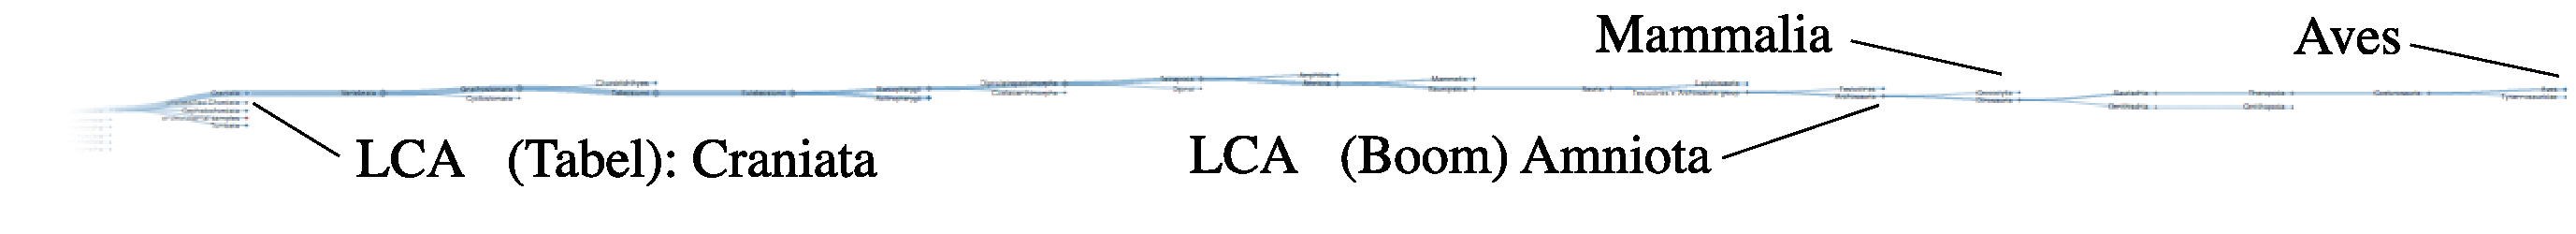
\includegraphics[width=1\textwidth]{includes/tabelanalyse}
    \caption{Weergave van \textit{Mammalia} en \textit{Aves} op de tak van de
    \textit{Craniata}. We zien dat de LCA op de tabel resulteert in
    \textit{Craniata}, terwijl de boomgebaseerde LCA de \textit{Amniota} vindt.
    Tussen de \textit{Craniata} en de \textit{Amniota} staan echter een tiental
    rangloze organismen. De boomgebaseerde taxonomische identificatie is dus een
    stuk specifieker.}
    \label{fig:boomvoorbeeld}
\end{figure}

\section{Boomgebaseerde LCA(*)} De hierboven genoemde reden is niet de enige
waarom het wenselijk is om een boomgebaseerde implementatie te maken. Zoals in
\Vref{chap:inleiding} beschreven is de laatste stap in de analyse om individuele
identificaties van alle peptiden uit een eiwit(fragment) of DNA read tot één
consensus te aggregeren.

In deze sectie diepen we het LCA* algoritme verder uit. We starten met een
implementatiebespreking van het gewone LCA algoritme en breiden die uit naar een
algoritme voor LCA*. Daarna bespreken we enkele problemen die voorkomen bij de
omvorming en hun oplossingen.

De berekening moet natuurlijk zo snel mogelijk verlopen. Daarom zouden we
dezelfde aanpak kunnen toepassen als Unipept om de LCA's van alle peptiden voor
te berekenen. Op die manier zouden we alle resultaten in een databank kunnen
opslaan, zodat we ze er in constante tijd uit kunnen halen. Die oplossing is
helaas onmogelijk door het gigantische aantal mogelijke combinaties van taxa die
als invoer kunnen worden gegeven. Er zijn op het moment van schrijven 1.267.511
taxa aanwezig in de NCBI taxonomy. Alle mogelijke subsets uit deze verzameling
voorberekenen zou onmogelijk zijn. Bij het voorberekenen van de LCAs van alle
peptiden (1.713.298.862) is dat wel mogelijk met voldoende opslagcapaciteit.

Iets wat we eventueel wel kunnen uitbuiten is de datastructuur waarop alle
analyses zullen uitgevoerd worden. Die is namelijk altijd dezelfde.

\subsection{Implementatie}
In deze sectie bespreken we een algoritme om de LCA van een opgegeven lijst van
nodes in een boomstructuur te berekenen. We tonen de tijd- en
ruimtecomplexiteiten van deze implementatie aan en bespreken vervolgens hoe we
het algoritme kunnen uitbreiden om als algoritme voor LCA* te gebruiken.

\subsubsection{State of the art}

Om het LCA probleem op te lossen, kijken we eerst naar de state of the art van
dit probleem. We baseren ons op het artikel ``Lowest Common Ancestors in Trees
and Directed Acyclic Graphs'' van Michael A. Bender en Martin Farach-Colton
\cites{lcabenderfarach}. In het artikel wordt een algoritme beschreven om het
LCA probleem in lineaire tijd te preprocessen. Dat kan door het LCA probleem om
te vormen naar een range minimum query (RMQ) probleem. Na preprocessing kan in
constante tijd de LCA van een paar nodes berekend worden.


\subsubsection{Van LCA naar RMQ}

Het LCA probleem is zoals we zien nauw verwant met het range minimum query (RMQ)
probleem. Het RMQ probleem  wordt geformuleerd als: 

\theoremstyle{definition}
\begin{definition}{RMQ}
Gegeven twee indices, $i$ en $j$, in lijst $A$, geef de index in $A$ van de 
kleinste waarde in de subarray $A[i..j]$''.
\end{definition}

Een belangrijke observatie hier is de volgende: de LCA van twee nodes, $u$ en
$v$, is de node die tijdens een Euler traversal van de boom tegenkomen wordt
tussen $u$ en $v$ met de kleinste diepte. Wanneer we dus van twee nodes, $u$ en
$v$, de LCA willen berekenen, kunnen we eerst een Euler traversal op de boom
uitvoeren waarbij we een lijst opstellen van dieptes van elke node die we
tegenkomen op dit pad. Een voorbeeld van een Euler traversal is uitgewerkt in
\Vref{tikz:eulertour}. De nodes worden met hun overeenkomstige diepte opgeslagen
in een tabel. De tabularire voorstelling van die Euler tour is te vinden in
\Vref{tbl:euler}.

\begin{figure}
    \centering
    \begin{tikzpicture}[node distance=2cm and 4cm, level distance=1.5cm, 
    sibling distance=10mm,
        every node/.style={draw, thick, circle,inner sep=5pt, node 
        distance=2cm},
        every path/.style={->, draw, thick, -latex'}]
    \Tree [. \node(nodeA){A}; 
             [. \node(nodeB){B}; ]
             [. \node(nodeC){C};
                [. \node(nodeE){E};
                   [. \node(nodeH){H}; ]
                   [. \node(nodeI){I}; ]
                ]
                [. \node(nodeF){F};
                   [. \node(nodeJ){J}; ]
                ] 
             ]
             [. \node[draw, fill=yellow](nodeD){D};
                [ . \node[draw, fill=red](nodeG){G}; ]
             ] 
          ]
          
    \draw[blue, dashed, ->] (nodeA.west) -- 
                             (nodeB.north);
    \draw[blue, dashed, ->] (nodeB.east) -- 
                             (nodeA.south);
    \draw[blue, dashed, ->] (nodeA.south) -- 
                             (nodeC.west);
    \draw[blue, dashed, ->] (nodeC.west) -- 
                             (nodeE.west);
    \draw[blue, dashed, ->] (nodeE.west) -- 
                             (nodeH.west);
    \draw[blue, dashed, ->] (nodeH.east) -- 
                             (nodeE.south);
    \draw[blue, dashed, ->] (nodeE.south) -- 
                             (nodeI.west);
    \draw[blue, dashed, ->] (nodeI.east) -- 
                             (nodeE.east);
    \draw[blue, dashed, ->] (nodeE.east) -- 
                             (nodeC.south);
    \draw[blue, dashed, ->] (nodeC.south) -- 
                             (nodeF.west);
    \draw[blue, dashed, ->] (nodeF.west) -- 
                             (nodeJ.west);
    \draw[blue, dashed, ->] (nodeJ.east) -- 
                             (nodeF.east);
    \draw[blue, dashed, ->] (nodeF.east) -- 
                             (nodeC.east);
    \draw[blue, dashed, ->] (nodeC.east) -- 
                             (nodeA.east);
    \draw[blue, dashed, ->] (nodeA.east) -- 
                             (nodeD.west);
    \draw[blue, dashed, ->] (nodeD.west) -- 
                             (nodeG.west);
    \draw[blue, dashed, ->] (nodeG.east) -- 
                             (nodeD.east);
    \draw[blue, dashed, ->] (nodeD.north) -- 
                             (nodeA.east);

    \end{tikzpicture}
    \caption{Illustratie van een Euler traversal door een boom. Hier duiden 
    blauwe pijlen het pad aan dat doorheen de boom genomen wordt. De tabulaire 
    voorstelling van dit pad is te vinden in \Vref{tbl:euler}.}
    \label{tikz:eulertour}
\end{figure}

\begin{table}
	\centering
	\caption{Tabulaire voorstelling van een Euler traversal door de boom uit 
	\Vref{tikz:eulertour}.}
	\label{tbl:euler}
   	\begin{tabular}{cccccccccccccccccccc}
       	\toprule
       	Index & 0 & 1 & 2 & 3 & 4 & 5 & 6 & 7 & 8 & 9 & 10 & 11 & 12 & 
       	13 & 14 & 15 & 16 & 17 & 18 \\ 
       	\midrule
       	Node   & A & B & A & C & E & H & E & I & E & C & F & J & F & C & A 
       	& D & G & D & A \\ 
       	Diepte & 0 & 1 & 0 & 1 & 2 & 3 & 2 & 3 & 2 & 1 & 2 & 3 & 2 & 1 & 
       	0 & 1 & 2 & 1 & 0 \\ 
       	\bottomrule
   	\end{tabular} 
   	\vspace{1cm}
   	\caption{Tabel van eerste voorkomens van een node in \Vref{tbl:euler}.}
   	\label{tbl:firstocc}
    \begin{tabular}{cccccccccc}
        \toprule
        A & B & C & D & E & F & G & H & I & J \\ 
        \midrule
        0 & 1 & 3 & 15 & 4 & 10 & 16 & 5 & 7 & 11  \\ 
        \bottomrule
    \end{tabular} 
\end{table}

Eenmaal die tabel is opgesteld, kunnen we het RMQ algoritme toepassen op het
deel tussen node $u$ en node $v$ van de tabel. Het deel tussen die nodes kunnen
we vinden door gebruik te maken van de tabel van eerste voorkomens, weergegeven
in \Vref{tbl:firstocc}. Door de bijhorende indices te nemen van node $u$ en $v$,
kunnen we in \Vref{tbl:euler} RMQ toepassen op de lijst van dieptes van nodes
tussen deze indices. Ter illustratie kunnen we bijvoorbeeld de LCA berekenen van
nodes I en J. Nodes I en J komen volgens de tabel van eerste voorkomens
respectievelijk voor in de Euler traversal tabel op positie 7 en 11. De nodes
tussen I en J zijn dus [I, E, C, F, J] met respectievelijke dieptes [3, 2, 1, 2,
3]. De node met de laagste diepte is dus C.

Formeel samengevat gaat de reductie van een LCA probleem naar een RMQ probleem
als volgt (waarbij $n$ het aantal nodes in de boom is):

\begin{enumerate}
\item Stel de \texttt{euler\_tour} array van lengte $2*n-1$ op die de identifier
van de nodes bevat als we de boom langs het Euleriaanse pad aflopen;

\item Stel de \texttt{levels} array van lengte $2*n-1$ op waarbij $depth_i$
overeen komt met de diepte van overeenkomstige node \texttt{euler\_tour[i]};

\item Stel de \texttt{first\_occurences} array op van lengte $n$ op, waarbij
$first\_occurences[i]$ overeen komt met het eerste voorkomen van node $i$ in
\texttt{euler\_tour}.
\end{enumerate}

Het opstellen van die drie arrays kan in één depth-first traversal door de boom 
gebeuren. De voorbeeldcode hiervoor is terug te vinden in \Cref{lst:dfsrun} op 
\cpageref{lst:dfsrun}.

\begin{lstlisting}[caption={Voorbeeldcode om het LCA probleem te reduceren naar 
een probleem dat met RMQ kan worden opgelost.}, label={lst:dfsrun}, 
language=Python, float]
def dfs_run(self, taxon, iteration, level):

    euler_tour[iteration] = taxon.taxon_id
    levels[iteration] = level
    if not first_occurences[taxon.taxon_id]:
        first_occurences[taxon.taxon_id] = iteration

    for child in taxon.children:
        iteration = dfs_run(child, iteration + 1, level + 1)

        euler_tour[iteration] = taxon.taxon_id
        levels[iteration] = level

    return iteration + 1

euler_tour = [None]*(2*tree.length)-1)
levels = [None]*(2*tree.length)-1)
first_occurences = [None]*tree.length

dfs_run(root_taxon, 0, 0)
\end{lstlisting}

Wanneer deze drie arrays opgesteld zijn, komt het vinden van de LCA van twee 
nodes $u$ en $v$ neer op het volgende:

\begin{enumerate}

\item Zoek de index van $u$ en $v$ in de \texttt{first\_occurences} array. Dit
geeft \texttt{first\_occurences[u]} en \texttt{first\_occurences[v]} die de
positie van het eerste voorkomen van respectievelijk $u$ en $v$ in de
\texttt{euler\_tour} en de \texttt{levels} array aanduidt;

\item Bereken de RMQ in de subarray van \texttt{levels} van
\texttt{first\_occurences[u]} tot\\
\texttt{first\_occurences[v]}:
$\text{RMQ}_{levels}$(\texttt{first\_occurences[u]}:\texttt{first\_occurences[v]}).
Het resultaat hiervan is de index van de node met de kleinste diepte in de 
Euler traversal tussen $u$ en $v$;

\item De LCA van $u$ en $v$ bevindt zich nu in de \texttt{euler\_tour} array op
de index van het resultaat van voorgaande RMQ-bewerking:\\ LCA(u, v) =
\texttt{euler\_tour}[$\text{RMQ}_{levels}$(\texttt{first\_occurences[u]}:\texttt{first\_occurences[v]})].

\end{enumerate}

\subsubsection{RMQ}
De omzetting van het LCA probleem naar een RMQ probleem is dus zeker mogelijk in
lineaire tijd ten opzichte van de nodes in de boom. RMQ zelf is echter geen
eenvoudig probleem. In deze paragraaf wordt van een triviale implementatie
vertrokken en wordt gaandeweg een meer optimale oplossing bekomen, gebruik
makend van een aantal lemma's en observaties.

Er wordt gestart van een array $A$ van lengte $n$ met de eigenschap dat elk
element met $\pm1$ verschilt van zijn buren. De $\pm1$ beperking ontstaat
aangezien we het RMQ algoritme gebruiken op de \texttt{levels} array uit het
voorgaande deel. Het RMQ probleem op arrays waar niet aan die eigenschap is
voldaan, zullen we vanaf nu het RMQ probleem noemen. Wanneer wel aan deze
eigenschap is voldaan, noemen we dat het RMQ$\pm1$ probleem. In beide gevallen
blijft het doel om, gegeven twee indexen in lijst $A$, $i$ en $j$, de index van
de kleinste waarde in $A$ te bekomen tussen $i$ en $j$, met $i$ en $j$
inclusief.

\paragraph{Naïeve oplossing}
De naïeve oplossing is een oplossing die alle mogelijke combinaties van $i$ en
$j$ voorberekent. Deze oplossing heeft een complexiteit van $\Theta(n^3)$ om
alles voor te berekenen wat kan worden gereduceerd tot $\Theta(n^2)$ door
gebruik te maken van dynamisch programmeren. Het uitvoeren van de effectieve RMQ
vereist één lookup en kan dus in constante tijd gebeuren. Een preprocessing stap
van $\Theta(n^2)$ is echter veel te traag, zeker aangezien er snellere
algoritmes bestaan.
\paragraph{Snellere oplossing voor het algemene RMQ probleem} 
Er bestaat een snellere oplossing voor het algemene RMQ probleem. Het algemene
idee is om elke mogelijke query voor te berekenen waarvan de lengte een macht
van 2 is. Bij het opzoeken kunnen we dan de range opdelen in 2 (eventueel
overlappende) blokken waarvan de lengte een macht van 2 is. Om in constante tijd
tot een antwoord te komen, moeten we dus eerst voor elke $i$ tussen 1 en $n$ en
elke $j$ tussen 1 en $\log{n}$ het kleinste element van de deelarray startend
bij $i$ met lengte $2^j$ berekenen. Het resultaat hiervan voeren we in in de
tabel $M$ op positie $[i,j]$.  Formeel wordt dit: $M[i,j] = \min{\{A[k], k = i
.. i + 2^j - 1\}}$. Zo hebben we voor elke mogelijke startindex alle mogelijke
blokken binnen de array van een lengte van een macht van twee, startend op die
index. Voorgaande berekening is het eenvoudigst te begrijpen aan de hand van een
voorbeeld: voor de rij $[1, 6, 2, 4]$  van lengte 4, geeft dit het volgende
effect:

{ \centering
{ \footnotesize
\begin{tabular}{x{2cm}x{2cm}x{2cm}x{3cm}}
1 & 6 & 2 & 4\\

\cline{1-1}
\multicolumn{1}{l}{$M[1,0]=\min{A[1..1]}$} &  &  &  \\
\cline{1-2}
\multicolumn{2}{l}{$M[1,1]=\min{A[1..2]}$} &  &  \\
\cline{1-4}
\multicolumn{4}{l}{$M[1,2]=\min{A[1..4]}$}\\

\cline{2-2}
& \multicolumn{1}{l}{$M[2,0]=\min{A[2..2]}$}  &  & \\
\cline{2-3}
& \multicolumn{2}{l}{$M[2,1]=\min{A[2..3]}$}  & \\
\cline{2-4}
& \multicolumn{3}{l}{$M[2,2]=\min{A[2..5]}$}  \\

\cline{3-3}
& & \multicolumn{1}{l}{$M[3,0]=\min{A[3..3]}$}  & \\
\cline{3-4}
& & \multicolumn{2}{l}{$M[3,1]=\min{A[3..4]}$} \\
\cline{3-4}
& & \multicolumn{2}{l}{$M[3,2]=\min{A[3..6]}$}  \\

& & & ... \\
\end{tabular}
}
}

Met behulp van bovenstaande illustratie wordt duidelijk ingezien dat de
volledige matrix $M$ kan worden opgebouwd via dynamisch programmeren.

Formeel kan deze tabel opgebouwd worden volgens de formules, waarbij $M[i,j]$ 
met $j = 0$ overeen komt met het element op positie $i$ in $A$. 
\begin{equation*}
M[i,j] =
\begin{cases}
 M[i, j - 1], & \text{als } A[M[i,j - 1]] \leq A[M[i+2^{j - 1}-1, j - 1]]\\
 M[i + 2^{j-1}-1, j-1], & \text{anders} 
\end{cases}
\end{equation*}

In woorden omgezet betekent dit dat we in een blok van lengte $2^j$ het minimum
kunnen nemen van de blokken van lengte $2^{j-1}$ waaruit dit blok van lengte
$2^j$ is opgebouwd. In bovenstaand voorbeeld kunnen we zo $M[1,1]$ vinden door
het minimum te nemen van $M[1,0]$ en $M[2,0]$. Op dezelfde wijze kan $M[3,1]$
gevonden worden door het minimum te nemen van $M[3,0]$ en $M[4,0]$. Om dan
$M[1,2]$ te vinden, nemen we het minimum van $M[1,1]$ en $M[3,1]$ die we zonet
berekend hebben. Deze tabel kan dus worden opgevuld in $\Theta(n\log{n})$ tijd
en ruimte.

Voor bovenstaand voorbeeld ziet die tabel er dan als volgt uit:

\begin{tabular}{r|ccc}
	\toprule
	i & $j=0$ & $j=1$ & $j=2$ \\
	\midrule
	1 &   0   &   0   & 0     \\
	2 &   1   &   2   & 2     \\
	3 &   2   &   2   & 2     \\
	4 &   3   &   3   & 3     \\
	\bottomrule
\end{tabular}\\

De RMQ van een range van $i$ tot $j$ in $A$ kan nu gevonden worden door twee
(eventueel) overlappende blokken die deze volledige subarray bedekken. Om dat te
bekomen zoeken we eerst het grootste blok met een lengte van een macht 2 dat
binnen de subarray past. De lengte van dat blok kan eenvoudig berekend worden
met de formule $2^{\lceil \log(j - i) \rceil}$. De RMQ van die subarray vinden
we dan door het minimum te nemen van de RMQ op het blok dat start op index $i$ 
en
de RMQ van het blok dat eindigt op index $j$. Aangezien deze blokken een lengte
van een macht van 2 hebben, heeft de preprocessing de minima van die blokken al
voorberekend en kunnen we dus de RMQ in constante tijd berekenen van deze
arbitraire subarray.

In bovenstaand voorbeeld kunnen we bijvoorbeeld de RMQ berekenen van index 0 
tot 2. Hiervoor selecteren we twee blokken met lengte $2^{\lceil \log(2 - 0) 
\rceil} = 2$. Het eerste blok start op index 0, het laatste blok eindigt op 
index 2. De RMQ van deze twee blokken is al voorberekend: $A[M[1,1]] = A[0] = 
1$ en $A[M[2,1]] = A[2] = 2$. De oplossing is dus 1, te vinden in A op index 0.

Dit algoritme kan dus de array $A$ voorberekenen in $\Theta(n\log{n})$ tijd en
ruimte. Opzoekingen kunnen als gevolg van deze voorberekening in constante
snelheid gebeuren.

\paragraph{Oplossing voor het RMQ$\pm1$ probleem}
Het voorberekenen kan echter nog sneller wanneer de array $A$ voldoet aan de
$\pm1$ beperking. In het geval van de \texttt{levels} array is dat altijd zo
aangezien we altijd van kind naar ouder of omgekeerd gaan.

Eerst wordt de array $A$ verdeeld in blokken ter grootte van
$\frac{\log{n}}{n}$. Daarna wordt een array, $A'$ gedefinieerd van
$\frac{2*n}{\log{n}}$ elementen, waarbij het element op index $i$ in $A'$ het
minimum element is van het $i^\text{de}$ blok in $A$. Aangezien het RMQ
algoritme de index van het kleinste element in een array teruggeeft en niet de
waarde zelf, wordt een bijhorende array gedefinieerd, $B$ waar $B_i$ de positie
aangeeft van het kleinste element in het $i^\text{de}$ blok van $A'$.

Nu kan voorgaand algoritme voor het algemene RMQ probleem toegepast worden op 
de nieuwe array $A'$. Aangezien $A'$ van lengte $\frac{2*n}{\log{n}}$ is en 
het RMQ algoritme een tijdscomplexiteit heeft van $n * \log{n}$, gebeurt dit in 
$\Theta\left[\frac{2*n}{\log{n}} * \log{\frac{2*n}{\log{n}}}\right] \approxeq 
\Theta(n)$ tijd.

Op basis van de huidige preprocessing van $A'$ kunnen alle combinaties van $i$
en $j$ in constante tijd gevonden worden wanneer $i$ en $j$ op de grenzen van de
blokken in A vallen. Dit is echter niet altijd het geval. Aangezien $i$ en $j$
binnen eenzelfde blok kunnen vallen, moeten we ook elk blok apart voorberekenen.
Het is echter ook mogelijk dat $i$ en $j$ in verschillende blokken vallen. In
dat geval wordt de RMQ als volgt berekend:

\begin{enumerate}
\item Bereken het minimum van $i$ tot het einde van het blok waar $i$ in valt;
\item Bereken het minimum van alle blokken in $A$ tussen de blokken waar $i$ en
$j$ in vallen; 
\item Bereken het minimum van $j$ tot het begin van het blok waar $j$ in valt.
\end{enumerate}

Het minimum van deze drie waarden is dan het kleinste element binnen de array
$A$ tussen $i$ en $j$. Om stap 2 te berekenen kan gebruik worden gemaakt van de
reeds voorberekende array $A'$. Stap 1 en 3 vergen echter wat meer werk. Er moet
nu een snelle manier worden gevonden om een RMQ probleem te beantwoorden
binnenin één blok.

Als op elk blok in $A$ apart de algemene RMQ preprocessing zou worden gedaan,
zouden we te veel tijd spenderen aan preprocessing. Daarom wordt gekeken of we
het aantal mogelijke blokken kunnen beperken. Dat kan ook volgens
volgende observatie: Wanneer twee arrays, $X$ en $Y$, beide van lengte $k$, op
elke positie met een constante waarde verschillen zodat $X_i = Y_i + c$ voor
elke $i$ en een constante $c$, dan zijn alle mogelijke RMQ antwoorden hetzelfde
voor beide arrays. Bijvoorbeeld gegeven arrays $[1, 2, 1, 0]$ en $[3, 4, 3, 2]$
dan geldt deze observatie voor $c = 2$. In beide blokken is het resultaat van de
RMQ voor het volledige blok gelijk, namelijk index 3.

Deze observatie heeft een belangrijk gevolg. Nu kunnen we namelijk elk blok 
normaliseren door de eerste waarde uit dat blok af te trekken van alle waarden 
in datzelfde blok. Voor het voorbeeld hierboven geeft dit
$[1-1, 2-1, 1-1, 0-1] = [3-3, 4-3, 3-3, 2-3] = [0, 1, 0, -1]$. 

Er kan nu worden aangetoond dat er $\Theta(\sqrt{n})$ verschillende
genormaliseerde blokken kunnen bestaan. Alle genormaliseerde blokken starten
namelijk met $0$ aangezien die waarde van zichzelf wordt afgetrokken. Wegens de
$\pm1$ beperking die ook op deze genormaliseerde blokken geldt, bekomen we
strings van lengte $\frac{\log{n}}{2} - 1$, waarbij $n$ nog steeds de lengte is
van de originele array $A$. Deze genormaliseerde blokken kunnen we ook omzetten
in bitstrings waarbij een 1 aangeeft dat het getal op die index 1 hoger is dan
zijn voorgaande getal, en 0 op dezelfde manier een verschil van -1 aangeeft. Dit
resulteert in het bestaan van $2^{\frac{\log{n}}{2} - 1} = \frac{\sqrt{n}}{2} =
\Theta(\sqrt{n})$ bitstrings, en dus $\Theta(\sqrt{n})$ mogelijke
genormaliseerde blokken.

Wat nu nog rest is het maken van tabellen voor elk genormaliseerd blok. Voor 
deze
$\Theta(\sqrt{n})$ blokken wordt een tabel aangemaakt waarin we alle antwoorden
voor RMQ opvragingen binnen dat blok opslaan. Dit zijn er $\frac{\log{n}}{2}^2 =
\Theta\left(\log{n}^2\right)$ per blok, dus
$\Theta\left(\sqrt{n}\log{n}^2\right) \approxeq \Theta(n)$ in totaal.
Opzoekingen kunnen aan de hand van deze tabellen in constante tijd gebeuren.

Het laatste wat ons nog rest is het berekenen van welk blok in de originele 
array $A$ bij welk genormaliseerd blok hoort. Dit kan eenvoudig door een 
mapping bij te houden van de bitstring na normalisatie.

Samengevat hebben we nu binnen een tijdscomplexiteit van $\Theta(n)$
alle mogelijke RMQ$\pm1$ vragen binnen blokken voorberekend, alsook alle RMQ
vragen over meerdere blokken heen in dezelfde tijd. Door die voorberekening
kunnen we in constante tijd de drie benodigde minima opvragen zoals hierboven
aangegeven, en kunnen we nu voor eender welke opgegeven indices $i$ en $j$ het
RMQ$\pm1$ probleem oplossen in $\Theta(1)$. 

De omzetting van LCA naar RMQ kan door middel van de depth-first traversal in
$\Theta(n)$ gebeuren en dient éénmalig te gebeuren om de benodigde arrays  voor
de RMQ preprocessing voor te berekenen. De opslag voor zowel de benodigde arrays
van de boomstructuur als voor de de interne arrays in de RMQ preprocessing
bedraagt $\Theta(n)$.

\paragraph{Implementatie} 

Aangezien er enkele C bibliotheken bestaan die bovenstaand algoritme voor het
RMQ probleem implementeren, zullen we gebruik maken van zo'n bestaande
bibliotheek. De bibliotheek die we hiervoor gebruiken is een implementatie
geschreven door Hideo Bannai \cite{Hideo0:online, Hideo1:online} die voldoet aan
de besproken snelheids- en ruimtecomplexiteiten. Het berekenen van de
LCA van twee nodes gebeurt dan zoals geïllustreerd in \Vref{lst:lcaexample}.

\begin{lstlisting}[language=Python, caption={Voorbeeldcode in Python voor de 
LCA berekening van 2 nodes, na uitvoering van \Vref{lst:dfsrun}},
label={lst:lcaexample}, float]
def calc_lca_pair(first, second):
    first_index = first_occurences[first]
    second_index = first_occurences[second]
    
    rmq_index = get_rmq(first_index, second_index)
    
    return euler_tour[rmq_index]
\end{lstlisting}

\subsubsection{LCA van meerdere nodes} 

Met voorgaand algoritme kan gemakkelijk de LCA van twee nodes berekend worden.
Het probleem wordt echter moeilijker wanneer we de LCA van meer dan twee nodes
willen berekenen.

In een boomstructuur waar een interne orde opgelegd is, zouden we de boom
in-order kunnen overlopen. Daarna kunnen we uit alle querynodes de twee nodes
opzoeken die het eerst en het laatst voorkomen tijdens deze in-order wandeling
door de boom. Dit garandeert dat de twee geselecteerde nodes de buitenste nodes
van alle querynodes zijn, en dat dus enkel de LCA van deze twee nodes moet
berekend worden om tot een eindresultaat te komen voor alle querynodes.

Met deze aanpak zijn er echter twee aspecten die we in rekening moeten brengen.
Ten eerste is het niet mogelijk een vaste volgorde op te leggen aan de taxa in
de NCBI taxonomy. Enkel de kind-ouder relatie bestaat hier. Hoe een kind zich
verhoudt ten opzichte van ouder of broers is niet vastgelegd. Het proberen
opstellen van een in-order volgorde van een ouder met twee kinderen, A en B, kan
dus resulteren in zowel [A, ouder, B] als [B, ouder, A]. Wanneer de LCA(A,
ouder, B) berekend wordt, zal afhankelijk van de volgorde LCA(A, B) of LCA(B, A)
berekend worden, wat wegens het symmetrisch zijn van LCA hetzelfde resultaat
oplevert.

Ook belangrijk is dat de taxonomische boom geen binaire boom is. Stel dat de
voorgaande ouder er nog een kind bij krijgt, C, dan kan het in-order overlopen
volgende volgordes aannemen: [A, ouder, B, C], [A, B, ouder, C], [C, B, ouder,
A], et cetera. Als we dan opnieuw de LCA berekenen van LCA(A, ouder, B) dan
weten we niet of we LCA(A, B), LCA(A, ouder), LCA(B, A), ... moeten berekenen.
Ook hier leveren alle mogelijkheden hetzelfde resultaat op, namelijk de ouder, 
maar
we zullen later zien dat dit bij het LCA* algoritme niet het geval is.

\subsection{Van LCA naar LCA*} 

De aanpassing van LCA naar LCA* lijkt op het eerste zicht vrij eenvoudig. Als we
de LCA berekenen van twee nodes, en het resultaat van deze berekening is één van
die twee nodes, dan weten we dat beide nodes op hetzelfde pad naar de wortel
liggen. Als resultaat nemen we dan de node met de grootste diepte in plaats van
deze met de kleinste diepte in het geval van LCA*. De code die de LCA berekent
uit \Vref{lst:lcaexample} wordt dan uitgebreid naar de code in
\Vref{lst:lca*example}.

\begin{lstlisting}[language=Python, caption={Uitbreinding van de voorbeeldcode 
uit \Vref{lst:lcaexample} in Python voor de LCA* berekening van 2 nodes}, 
label={lst:lca*example}, float]
def calc_lca_pair(first, second):
    first_index = first_occurences[first]
    second_index = first_occurences[second]
    
    rmq_index = get_rmq(first_index, second_index)
    
    # Speciaal geval LCA*
    if rmq_index == first_index:
        lca_index = second_index
    elif rmq_index == second_index:
        lca_index = first_index
    # Wanneer de RMQ index geen van beide originele indexen is, gebruik LCA
    else:
        lca_index = rmq_index
    
    return euler_tour[lca_index]
\end{lstlisting}

Deze aanpassing levert echter problemen op voor het toepassen van het LCA*
algoritme wanneer de LCA wordt berekend van meer dan twee nodes. Zoals uitgelegd
in de vorige sectie, kan de LCA van meer dan twee nodes gevonden worden door het
LCA algoritme toe te passen op de eerste en laatste querynode bij een in-order
overlopen van de boom.

Stel dat we de boom er terug bij nemen met een ouder en drie kinderen: A, B en C
en de ordening [A, B, ouder, C]. LCA*(ouder, A, B) met de methode van het nemen
van de ``buitenste'' querynodes reduceert het probleem naar LCA*(A, ouder) wat
met voorgaand algoritme resulteert in A. Hier is echter de informatie uit de tak
van B verdwenen, A kan namelijk nooit het resultaat zijn van LCA*(A, B). Ook een
pre- en post-ordening hebben hetzelfde probleem, aangezien er geen specifieke
ordening vast ligt voor de taxonomische boom. Bijvoorbeeld met de pre-ordening
[ouder, A, B, C] is de LCA*(ouder, B, C) = LCA*(ouder, C) = C, waarbij de tak
van B opnieuw onterecht wordt genegeerd. Als laatste middel kunnen we nog terug
proberen te vallen op de Eulertraversal ordening, [ouder, A, ouder, B, ouder, C,
ouder], maar ook hier geldt het tegenvoorbeeld: LCA*(ouder, A, B) = LCA*(ouder,
B) = B, waarbij ditmaal de tak van A genegeerd wordt.

Een alternatief is het paarsgewijs toepassen van het LCA*-algoritme. Gegeven een
lijst van nodes kunnen we eerst voor de eerste twee nodes in die lijst de LCA*
berekenen. Het resultaat daarvan kan dan met LCA* geaggregeerd worden met de
derde node in de lijst. Op deze manier worden verder gegaan tot alle nodes in de
lijst zijn geaggregeerd. Grote lijsten kunnen op die manier zelfs parallel
verwerkt worden. Zo kan LCA*(A, B, C, D) bijvoorbeeld berekend worden aan de
hand van LCA*(LCA*(A, B), LCA*((C, D)). Voor het klassieke LCA-algoritme werkt
dit probleemloos aangezien we nooit in de boom afdalen. Dit is echter niet het
geval bij het LCA*-algoritme. In \Vref{fig:lca*hij} berekenen we bijvoorbeeld
LCA*(H, I, J). Dit wordt paarsgewijs berekend door eerst LCA*(H, I) = E te
berekenen en daarna LCA*(E, J) = C. Wanneer we echter een verkeerd
tussenresultaat op hetzelfde pad als een volgende node bekomen, zoals in
\Vref{fig:lca*bcd}, dan kan dit een verkeerd resultaat opleveren. LCA*(B, C, D)
wordt berekend aan de hand van LCA*(B, C) = A, en daarna LCA*(A, D). Dit levert
dat de lager liggende node D als LCA* resultaat, waardoor de takken van B en C
volledig genegeerd worden en het resultaat eveneens fout is.

\begin{figure}
	\centering
    \begin{subfigure}{0.45\linewidth}
        \centering
        \begin{tikzpicture}[node distance=3cm, level distance=1.5cm,
            every node/.style={draw, thick, circle,inner sep=5pt},
            every path/.style={->, draw, thick, -latex'}]
        \Tree [. A 
                 [. B ]
                 [. C
                    [. \node[draw, fill=green]{E};
                       [. \node[draw, fill=yellow]{H}; ]
                       [. \node[draw, fill=yellow]{I}; ]
                    ]
                    [. F
                       [. \node[draw, fill=yellow]{J}; ]
                    ] 
                 ]
                 [. D
                    [ . G ]
                 ] 
              ]
        \end{tikzpicture}
        \caption{}
        \label{tikz:lca*hij}
    \end{subfigure}
    \begin{subfigure}{0.45\linewidth}
        \centering
        \begin{tikzpicture}[node distance=3cm, level distance=1.5cm,
            every node/.style={draw, thick, circle,inner sep=5pt},
            every path/.style={->, draw, thick, -latex'}]
        \Tree [. A 
                 [. B ]
                 [. \node[draw, fill=red]{C};
                    [. \node[draw, fill=green]{E};
                       [. \node[draw, fill=yellow]{H}; ]
                       [. \node[draw, fill=yellow]{I}; ]
                    ]
                    [. F
                       [. \node[draw, fill=green]{J}; ]
                    ] 
                 ]
                 [. D
                    [ . G ]
                 ] 
              ]
        \end{tikzpicture}
        \caption{}
        \label{tikz:lca*hij2}
    \end{subfigure}
    \caption{Tussenstappen voor berekenen van  LCA*(H, I, J). Gele nodes zijn
    querynodes, groene tussenresultaten en rode het eindresultaat. Via de
    iteratieve reductie geeft dit LCA*(LCA*(H, I), J), wat resulteert in LCA*(E,
    J). Het uitrekenen hiervan geeft C als correct resultaat.} 
    \label{fig:lca*hij}
\end{figure}

\begin{figure}
	\centering
    \begin{subfigure}{0.33\linewidth}
        \centering
        \begin{tikzpicture}[node distance=3cm, level distance=1.5cm,
            every node/.style={draw, thick, circle,inner sep=5pt},
            every path/.style={->, draw, thick, -latex'}]
        \Tree [. \node[draw, fill=green]{A}; 
                 [. \node[draw, fill=yellow]{B}; ]
                 [. \node[draw, fill=yellow]{C};
                    [. E
                       [. H ]
                       [. I ]
                    ]
                    [. F
                       [. J ]
                    ] 
                 ]
                 [. \node[draw, fill=yellow]{D};
                    [ . G ]
                 ] 
              ]
        \end{tikzpicture}
        \caption{}
        \label{tikz:lca*bcd1}
    \end{subfigure}
    \begin{subfigure}{0.33\linewidth}
        \centering
        \begin{tikzpicture}[node distance=3cm, level distance=1.5cm,
            every node/.style={draw, thick, circle,inner sep=5pt},
            every path/.style={->, draw, thick, -latex'}]
        \Tree [. \node[draw, fill=green]{A}; 
                 [. \node[draw, fill=yellow]{B}; ]
                 [. \node[draw, fill=yellow]{C};
                    [. E
                       [. H ]
                       [. I ]
                    ]
                    [. F
                       [. J ]
                    ] 
                 ]
                 [. \node[draw, fill=green]{D};
                    [ . G ]
                 ] 
              ]
        \end{tikzpicture}
        \caption{}
        \label{tikz:lca*bcd2}
    \end{subfigure}
    \begin{subfigure}{0.33\linewidth}
        \centering
        \begin{tikzpicture}[node distance=3cm, level distance=1.5cm,
            every node/.style={draw, thick, circle,inner sep=5pt},
            every path/.style={->, draw, thick, -latex'}]
        \Tree [. \node[draw, fill=green]{A}; 
                 [. \node[draw, fill=yellow]{B}; ]
                 [. \node[draw, fill=yellow]{C};
                    [. E
                       [. H ]
                       [. I ]
                    ]
                    [. F
                       [. J ]
                    ] 
                 ]
                 [. \node[draw, fill=red]{D};
                    [ . G ]
                 ] 
              ]
              
              
        \end{tikzpicture}
        \caption{}
        \label{tikz:lca*bcd3}
    \end{subfigure}
    \caption{Tussenstappen voor het berekenen van LCA*(B, C, D). Gele nodes zijn
    querynodes, groene tussenresultaten en rode het eindresultaat. Via de
    iteratieve methode geeft dit LCA*(LCA*(B, C), D), wat resulteert in LCA*(A,
    D). Het uitwerken van LCA*(A, D) geeft echter foutief D als resultaat
    waarbij de takken van B en C volledig genegeerd worden.}
    \label{fig:lca*bcd}
\end{figure}

De oorzaak van het probleem is te wijten aan het afdalen in de boom met het LCA*
algoritme wanneer een eerder bekomen LCA* resultaat als tussenstap gebruikt
wordt. Om dit probleem op te lossen, kan gebruik gemaakt worden van een
dieptelimiet in de boom, waar niet onder mag worden afgedaald. Deze dieptelimiet
schuift telkens op naar het niveau van een node die het resultaat is van een
LCA* tussenstap waar niet wordt afgedaald. In het voorbeeld in
\Vref{tikz:lca*bcd2} zou bij de berekening van LCA*(B, C, D) = LCA*(LCA*(B, C),
D) er na het verkrijgen van A als tussenresultaat van LCA*(B, C) dus niet verder
mogen worden afgedaald worden in een tak onder A, aangezien A reeds het
tussenresultaat is van een gewone LCA stap op B en C. Na deze stap wordt de
dieptelimiet op 0 gezet, aangezien resultaat A diepte 0 heeft. Wanneer een
volgende LCA* stap gedaan wordt op A en D, met dieptelimiet 0, dalen we niet af
naar D aangezien de diepte van D (1) groter is dan deze limiet (0). Dit wordt
geïllustreerd in \Vref{tikz:lcafix*bcd}. De nieuwe notatie die we hiervoor
invoeren is $\text{LCA}_d$* waarbij $d$ de huidige waarde is van de
dieptelimiet. LCA*($n_1$,$n_2$,...,$n_m$) is dan een korte notatie voor 
$\text{LCA}_\infty$*($n_1$,$n_2$,...,$n_m$).

\begin{figure}
	\centering
    \begin{subfigure}{0.33\linewidth}
        \centering
        \begin{tikzpicture}[node distance=3cm, level distance=1.5cm,
            every node/.style={draw, thick, circle,inner sep=5pt},
            every path/.style={->, draw, thick, -latex'}]
        \Tree [. \node[draw, fill=green]{A}; 
                 [. \node[draw, fill=yellow](nodeB){B}; ]
                 [. \node[draw, fill=yellow]{C};
                    [. E
                       [. \node(nodeH){H}; ]
                       [. I ]
                    ]
                    [. F
                       [. J ]
                    ] 
                 ]
                 [. \node[draw, fill=yellow](nodeD){D};
                    [ . G ]
                 ] 
              ]
              
          \draw[red, dashed, -] 
              (nodeH.south -| nodeB.west) -- 
              (nodeH.south -| nodeD.east);
        \end{tikzpicture}
        \caption{}
        \label{tikz:lcafix*bcd1}
    \end{subfigure}
    \begin{subfigure}{0.33\linewidth}
        \centering
        \begin{tikzpicture}[node distance=3cm, level distance=1.5cm,
            every node/.style={draw, thick, circle,inner sep=5pt},
            every path/.style={->, draw, thick, -latex'}]
        \Tree [. \node[draw, fill=green](nodeA){A}; 
                 [. \node[draw, fill=yellow](nodeB){B}; ]
                 [. \node[draw, fill=yellow](nodeC){C};
                    [. E
                       [. \node(nodeH){H}; ]
                       [. I ]
                    ]
                    [. F
                       [. J ]
                    ] 
                 ]
                 [. \node[draw, fill=green](nodeD){D};
                    [ . G ]
                 ] 
              ]
              
            \draw[red, dashed, -] 
                (nodeA.south -| nodeB.west) -- 
                (nodeA.south -| nodeD.east);
        \end{tikzpicture}
        \caption{}
        \label{tikz:lcafix*bcd2}
    \end{subfigure}
    \begin{subfigure}{0.33\linewidth}
        \centering
        \begin{tikzpicture}[node distance=3cm, level distance=1.5cm,
            every node/.style={draw, thick, circle,inner sep=5pt},
            every path/.style={->, draw, thick, -latex'}]
        \Tree [. \node[draw, fill=red](nodeA){A}; 
                 [. \node[draw, fill=yellow](nodeB){B}; ]
                 [. \node[draw, fill=yellow](nodeC){C};
                    [. E
                       [. H ]
                       [. I ]
                    ]
                    [. F
                       [. J ]
                    ] 
                 ]
                 [. \node[draw, fill=yellow](nodeD){D};
                    [ . G ]
                 ] 
              ]
              
              \draw[red, dashed, -] 
                  (nodeA.south -| nodeB.west) -- 
                  (nodeA.south -| nodeD.east);
              
        \end{tikzpicture}
        \caption{}
        \label{tikz:lcafix*bcd3}
    \end{subfigure}
    \caption{Tussenstappen voor het berekenen van $\text{LCA}_\infty$*(B, C, D).
    Gele nodes zijn querynodes, groene tussenresultaten en rode het
    eindresultaat. Met de paarsgewijze methode geeft dit 
    $\text{LCA}_0$*($\text{LCA}_\infty$*(B, C), D). De binnenste LCA* 
    berekening geeft A als resultaat. Aangezien B en C beide 
    deeltakken zijn van A wordt de dieptelimiet naar boven geschoven tot op de 
    diepte van A, namelijk 0. Dit resulteert in $\text{LCA}_0$*(A, D). Het 
    uitwerken hiervan zou met de oude methode D als resultaat geven, maar 
    aangezien de diepte van D groter is dan de dieptelimiet geven we A als 
    resultaat.}
    \label{tikz:lcafix*bcd}
\end{figure}

We breiden nu het codevoorbeeld uit \Vref{lst:lca*example} uit naar 
\Vref{lst:lcafix*example}, waarin rekening wordt gehouden met de dieptelimiet.

\begin{lstlisting}[language=Python, caption={Uitbreinding van de voorbeeldcode 
uit \Vref{lst:lca*example} in Python voor de LCA* berekening van 2 nodes. Deze 
code houdt rekening met de toegevoegde \texttt{depth\_limit} parameter. Zoals 
besproken kan de \texttt{reduce} stap hier ook geparallelliseerd worden in 
plaats van met een accumulator te werken.}, 
label={lst:lcafix*example}]
def calc_lca_pair(acc, second, depth_limit):
    depth_limit, first = acc

    first_index = first_occurences[first]
    second_index = first_occurences[second]
    
    rmq_index = get_rmq(first_index, second_index)
    
    # Speciaal geval LCA*
    if rmq_index == first_index and levels[second_index] <= depth_limit:
        lca_index = second_index
    elif rmq_index == second_index and levels[first_index] <= depth_limit:
        lca_index = first_index
    # Wanneer de RMQ index geen van beide originele indexen is, gebruik LCA
    else:
        lca_index = rmq_index
        depth_limit = levels[lca_index]
    
    return (euler_tour[lca_index], depth_limit)
    

# Input: een lijst (of generator) van taxon identifiers
taxon_ids = iter([...])

first = next(taxon_ids)
depth_limit = sys.maxsize

_, lca_id = reduce(calc_lca_pair, taxon_ids, (depth_limit, first))

\end{lstlisting}

\section{Toekomstig werk}

In dit hoofdstuk bespraken we een nieuwe aggregatiemethode om verschillende taxa
te aggregeren tot een zo specifiek mogelijk eindresultaat om te gebruiken bij de
analyse van metagenomic samples. Deze nieuwe methode moet natuurlijk wel ergens
kunnen worden gebruikt. De aangewezen plaats is hiervoor zijn de Unipept web
services, zodat deze door zowel de Unipept command-line interface als door de
webinterface kan gebruikt worden. In deze webservices is inmiddels al het
commando \texttt{taxa2lca}\cite{taxa2lca:online} ingebouwd, die gebruik maakt
van de huidige tabelgebaseerde berekening. Analoog aan dit commando zou dus een
nieuwe commando, \texttt{taxa2treelca} kunnen worden ingebouwd.  Aangezien alle
calls naar deze services zo snel mogelijk moeten gebeuren, zou het dus
aangeraden zijn dat de Unipept webservices de benodigde data voor het RMQ
probleem in memory houden zodat een LCA* vraag onmiddellijk kan worden
beantwoord zonder dat er nog iets moet worden opgestart of opgebouwd.

Als alternatief voor onderzoekers die hun data niet graag over het internet
sturen kunnen we ook een lokale versie van dit commando aanbieden. Dit houdt
natuurlijk wel in dat de gebruiker de benodigde arrays en preprocessing lokaal
moet doen. Voor de case study in \Vref{chap:casestudy} werden al enkele scripts
geschreven die een taxonomie kunnen inladen en deze omzetten in de benodigde
arrays en datastructuren om het LCA* probleem te kunnen oplossen. De gebruiker
zou er dan voor kunnen kiezen om zelf een service te draaien die deze
datastructuren in memory houdt, of om de voorberekende data te serialiseren
zodat deze niet telkens opnieuw hoeft voorberekend te worden.

Een laatste puntje dat verbeterd kan worden is het gebruik van de C bibliotheek.
Momenteel wordt deze vanuit Python opgeroepen, waardoor bij elke oproep naar die
bibliotheek de data moet worden omgezet van een Python datastructuur naar een C
datastructuur. Aangezien de Unipept web en command-line interface in Ruby
geschreven zijn zou die omzetting daar dus ook moeten gebeuren. Een
herimplementatie van die bibliotheek in native Python/Ruby code zou deze
omzetting, en dus ook het tijdsverlies dat ermee gepaard gaat, overbodig maken.
Of de resulterende native code dan ook werkelijk sneller is dan de omzetting
naar en de berekening in C zal gebenchmarkt moeten worden.